\chapter{\textbf{Procesamiento de datos}}
\label{cha:procesamiento_datos}

En esta sección describiremos el proceso que realiza el modelo tanto para el etiquetado de datos de entrenamiento con OLMO 3 así como para el procesamiento de etiquetado de datos realizado por ModernBERT, sus arquitecturas, ventajas sobre otros modelos, parametros, diferencias con las arquitecturas tradicionales, entre otros aspectos.


\section{Modelo OLMO 3 base}
OlMO 3, Modelo de lenguaje y pensamiento completamente abierto, con un modelo BASE y versiones mas complejas de THINK, INSTRUCT y RL-Zero, y con variaciones de 7B y 32B de parámetros, es un modelo de lenguaje desarrollado por Team OMLO \cite{olmo2025olmo3} aproximadamente 1 año de publicado el modelo OLMO 2 \textcite{groeneveld2025olmo2} en 2024. OLMO 3 posee muchas capacidades, tales como rasonamiento de largo contexto, código, seguimiento de insdtrucciones, etc. mantiene rendimiento de longitudes de contexto extendidas sobre los 65.000 tokens. 


\begin{figure}[H]
    \centering
    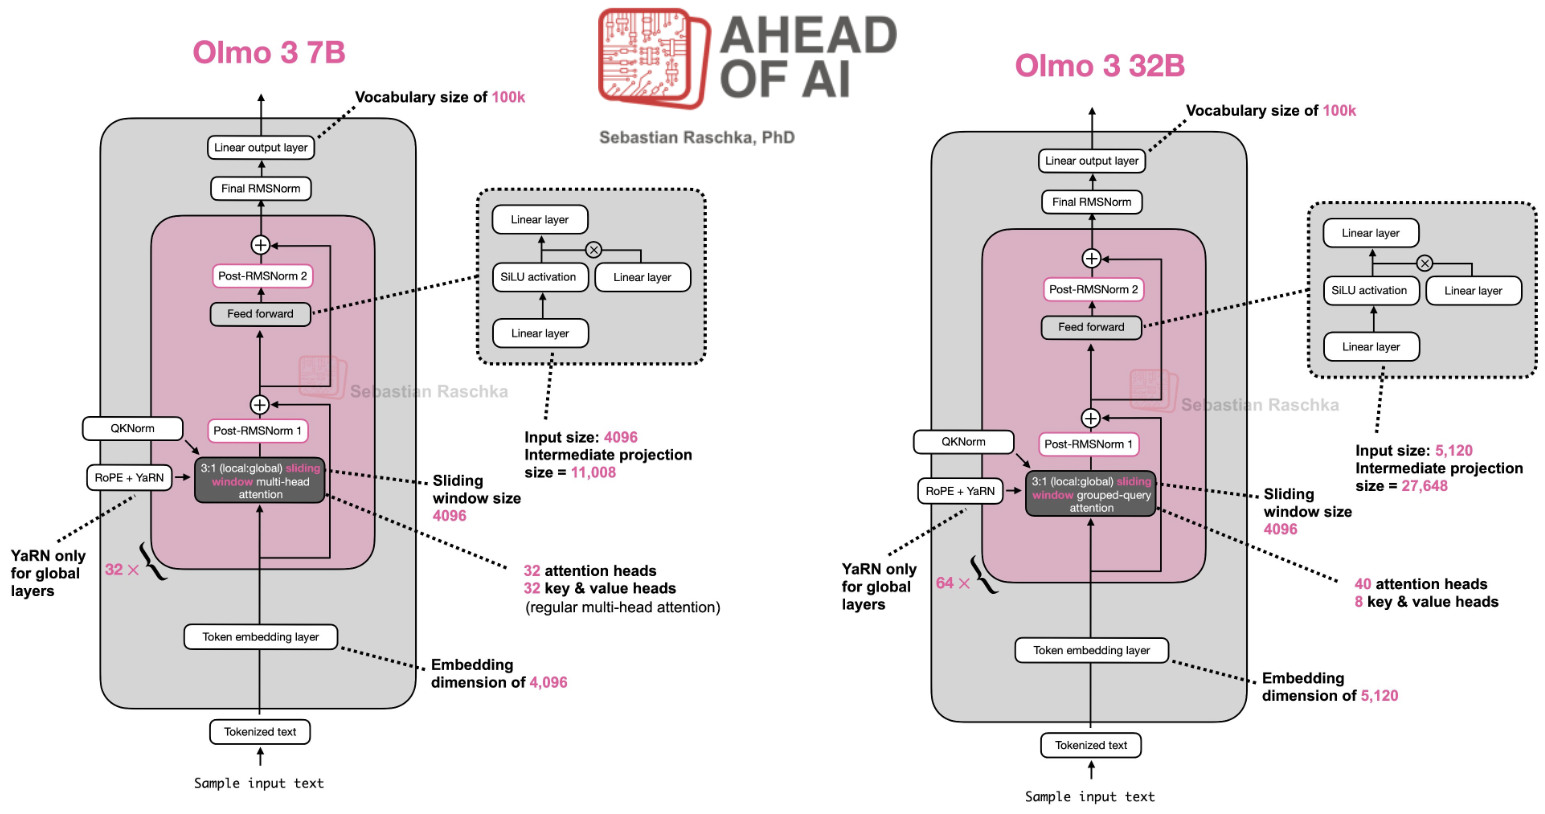
\includegraphics[width=\textwidth]{assets/Ejemplo Arquitectura OLMO 7 32.jpg}
    \caption{Resumen de arquitectura OLMO 3 7B vs 32B. Imagen extraida de \textcite{wolfe2025olmo3}}
    \label{fig:ResumenArquitecturaOLMO}
\end{figure}

\begin{figure}[H]
    \centering
    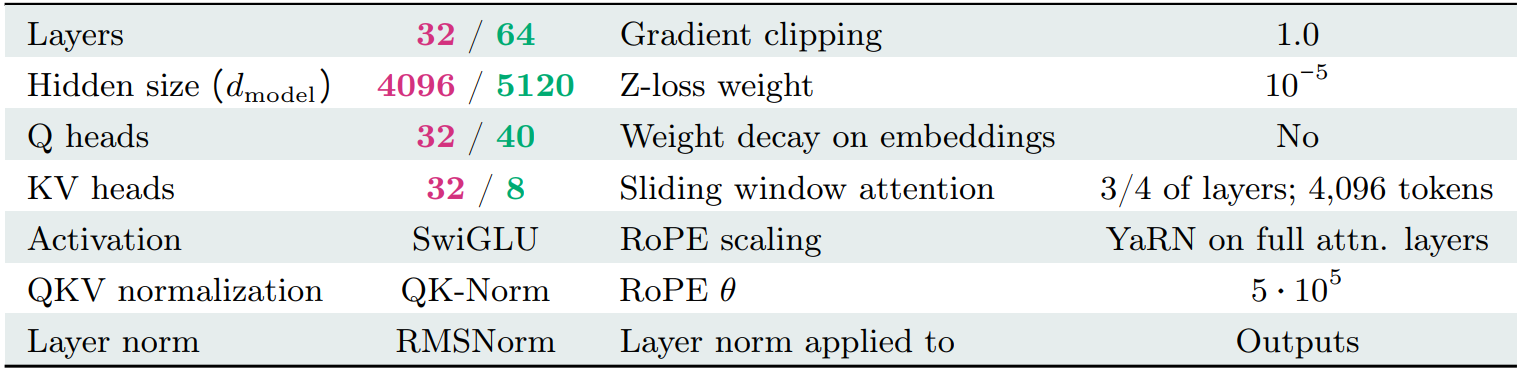
\includegraphics[width=\textwidth]{assets/Arquitectura 7B vs 32B.png}
    \caption{Arquitectura de OLMO 3 7B vs 32B. Imagen extraida de \textcite{olmo2025olmo3}}
    \label{fig:Arquitectura7Bvs32B}
\end{figure}

OLMO 3 corresponde a un tipo de modelo que adopta la arquitectura de Transformers de Solo Decodificadores (Decoder-Only Transformer por su traducción al inglés) definida en \textcite{vaswani2017attention}, donde el modelo de 7B de parámetros utiliza atencion de multiples cabezales (Multi Head Attention) siendo este el metodo estandar de trabajo de Transformers tradicionales para la \textit{"Atención"}, mientras que el modelo de 32B utiliza attencion a consultas agrupadas (grouped query attention) \textcite{ainslie-etal-2023-gqa} que a diferencia de la atención de múltiples cabezales, reduce el uso de memoria (enfocado a modelos grandes) al compartir cada grupo de cabezales un único par key/value por conjunto.\\

\begin{figure}[H]
    \centering
    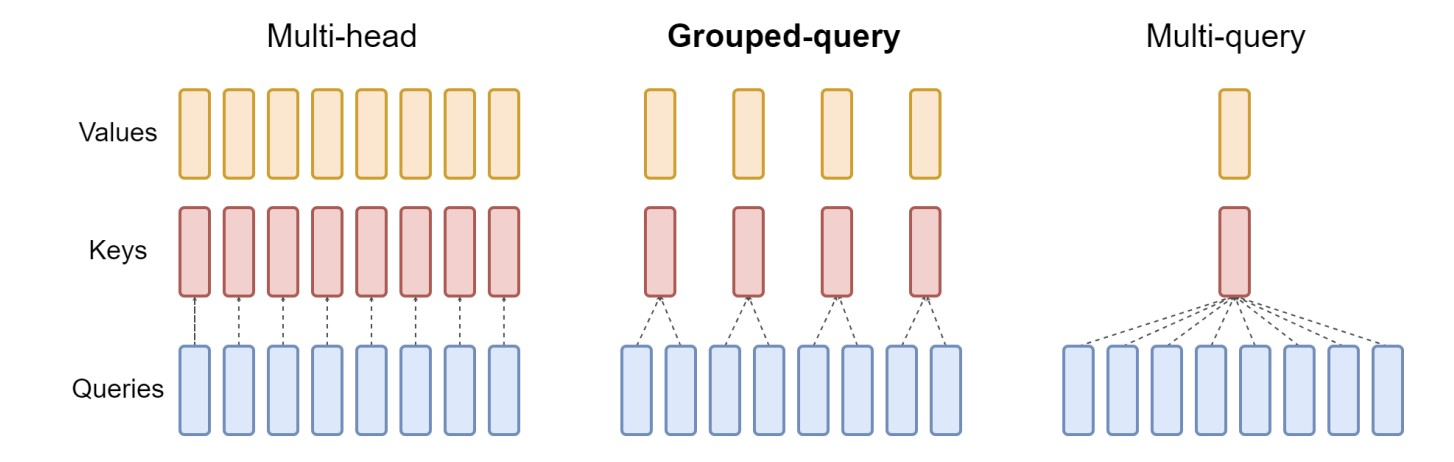
\includegraphics[width=\textwidth]{assets/MultiHead-GroupedQuery.jpg}
    \caption{Multi Head Attention vs Grouped Query Attention. Imagen extraida de \textcite{olmo2025olmo3}}
    \label{fig:MHeadGQuery}
\end{figure}

Como se puede observar en la figura \ref{fig:MHeadGQuery}, la diferencia entre Multi Head Attention (MHA) y Grouped Query Attention (GQA) radica en los pares key/value, mencionado previamente, mientras que en MHA cada cabeza de atención tiene su propio par key/value, en GQA cada grupo de cabezas comparte un único par key/value. Esto permite a GQA reducir el uso de memoria, lo que es especialmente beneficioso para modelos grandes como el OLMO 3 de 32B de parámetros. Sin embargo, es importante destacar que esta reducción en el uso de memoria puede llegar a ser perjudicial para el rendimiento del modelo. 



\section{Modelo OLMO 3 THINKING}

Pese a que el modelo OLMO 3 BASE posee un diseño de arquitectura similar, el modelo OLMO 3 THINKING (Considerando que comparamos ambos con la misma cantidad de parámetros), posee una diferencia pero no de arquitectura como tal, el modelo Thinking recibió un proceso de post-entrenamiento especializado para poder otorgarle la capacidad de "Pensar" de manera compleja.\\

Mientra que la arquitectura física, cabezales, parámetros, capas, neuronas, etc, se definen en el modelo OLMO 3 BASE mencionado en la figura \ref{fig:Arquitectura7Bvs32B}, el modelo OLMO 3 THINKING recibe un post-entrenamiento especializado, donde se le otorgan tareas de razonamiento complejo, como por ejemplo, razonamiento de múltiples pasos, razonamiento de largo contexto, razonamiento de código, etc. Esto permite que el modelo THINKING pueda comprender y procesar información de manera más profunda y compleja, lo que es especialmente útil para tareas que requieren un alto nivel de comprensión y análisis.\\








Prompt junto con \ref{cha:OLLAMA} y \ref{cha:MLX}




Para esta investigación se ha optado por utilizar el modelo Thinking de OLMO 3 de 7B de parámetros debido tanto a la necesidad del "pensamiento" y raciocinio necesarios para que el modelo comprenda cuando está en presencia de una sugerencia, así como por la cantidad de parámetros que posee (significando un menor costo computacional para la infraestructura disponible). \\

Pese a que la selección del modelo se vió restringida por el hardware que se tuvo a disposición al momento de la realización de las pruebas de etiquetado, no se descarta, si no que se espera poder realizar pruebas con una infraestructura significativamente mas potente, capaz de poder etiquetar con el modelo de 32B de parámetros, en un tiempo no superior a 1 semana, todos los datos disponibles dentro del dataset (Aproximdamente 560K de comentarios), lo que permitiría comparar los resultados obtenidos, con distintas combinaciones de modelos e infraestructura.\\




Cuantizado








\begin{figure}[H]
    \centering
    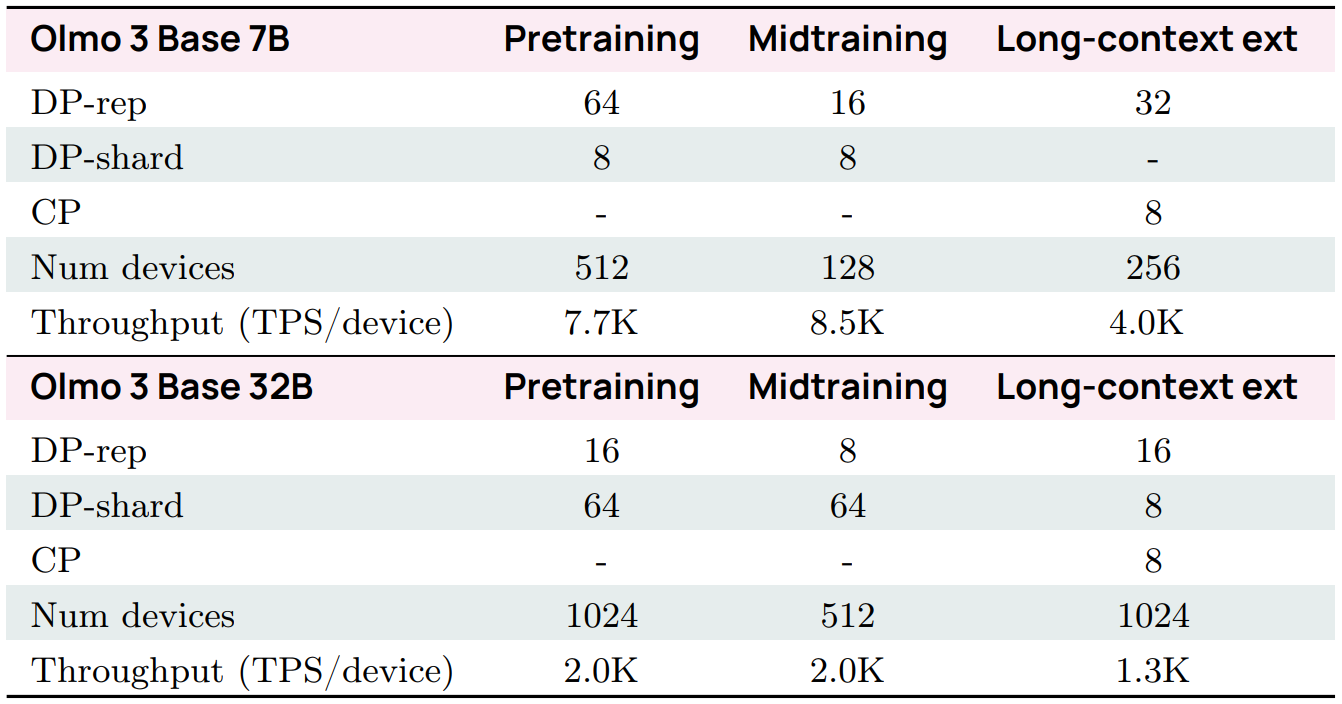
\includegraphics[width=\textwidth]{assets/Configuraciones de entrenamiento OLMO BASE 7B 32B.png}
    \caption{Configuraciones de entrenamiento OLMO BASE 7B 32B. Imagen extraida de \textcite{olmo2025olmo3}}
    \label{fig:ConfiguracionesEntrenamientoOLMO}
\end{figure}